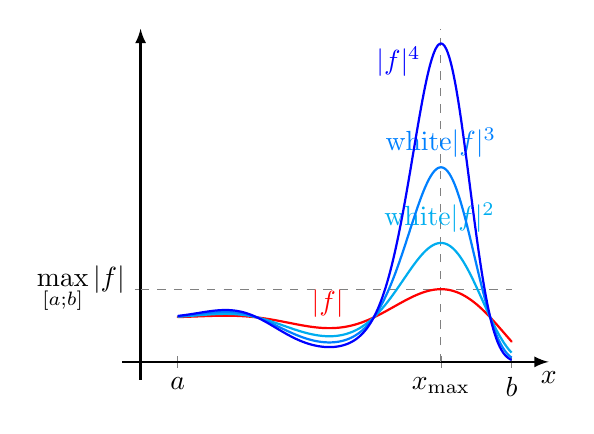
\begin{tikzpicture}
    \begin{axis}[
        width=7cm,
        xmin=-0.05, xmax=1.1,
        ymin=-0.4, ymax=7.5,
        axis lines=middle,
        axis line style=thick,
        axis line style={-latex},
        legend cell align={left}, 
        legend style={
            draw=none,
            fill=none,
            font=\footnotesize,
            legend image code/.code={\node[anchor=west] {#1};}
        },
        xtick={0.1, 0.8093645484949833, 1},
        xticklabels={$a$, $x_\mathrm{max}$, $b$},
        ytick={0, 1.6363476181939256},
        yticklabels={$0$, $\max\limits_{[a;b]} |f|$},
        xlabel=$x$,
        every axis x label/.style={at={(current axis.right of origin)},anchor=north},
    ];

    \draw[gray, dashed] (0,1.6363476181939256) -- (1,1.6363476181939256);
    \draw[gray, dashed] (0.8093645484949833,0) -- (0.8093645484949833,7.5);
    % Plot for n=1
    \addplot[domain=0.1:1, samples=200, color=red, smooth, thick, line join=round,line cap=round] {abs(x^2 * sin(10*deg(x))+1)} node[pos=0.2, above] {$|f|$};
    % \addlegendentry{\textcolor{blue!20!cyan}{$n = 1$}}

    % Plot for n=2
    \addplot[domain=0.1:1, samples=200, color=blue!0!cyan, smooth, thick] {abs(x^2 * sin(10*deg(x))+1)^2} node[pos=0.537, above] {\contour{white}{$|f|^2$}};
    % \addlegendentry{\textcolor{blue!40!cyan}{$n = 2$}}

    % Plot for n=3
    \addplot[domain=0.1:1, samples=200, color=blue!50!cyan, smooth, thick] {abs(x^2 * sin(10*deg(x))+1)^3} node[pos=0.533, above] {\contour{white}{$|f|^3$}};
    % \addlegendentry{\textcolor{blue!60!cyan}{$n = 3$}}

    % Plot for n=4
    \addplot[domain=0.1:1, samples=200, color=blue!100!cyan, smooth, thick] {abs(x^2 * sin(10*deg(x))+1)^4} node[pos=0.5, left] {$|f|^4$};
    % \addlegendentry{\textcolor{blue!80!cyan}{$n = 5$}}
    \end{axis}
\end{tikzpicture}
